\documentclass[12pt]{article}


%%%%%%%%%%%%%%%%%%%%%%%%%%%%%%%%%%%%%%%%%%%%%%%%%%%%%%%%%%%%%%%%%%%%%%%%%%%%%%%%%%%%%%
%%%%%%%%%%%%%%%%%%% YOU PROBABLY DON"T NEED TO CHANGE ANYTHING HERE %%%%%%%%%%%%%%%%%%%
\usepackage{amsfonts, amsmath} 
\usepackage{graphicx}
\usepackage{libertine} 
\usepackage{fullpage}
\usepackage{hyperref}
\usepackage{multicol}   % added: two-column reference list
% --- added: APA 7 citations and references (replaces natbib) ---
\usepackage[american]{babel}
\usepackage{csquotes}
\usepackage[style=apa,backend=biber]{biblatex}
\addbibresource{references.bib}
\setlength{\bibitemsep}{0pt}
\hypersetup{
    colorlinks = true,
    linkcolor = blue,
    urlcolor  = blue,
    citecolor = blue,
    anchorcolor = blue}
\urlstyle{same}
%%%%%%%%%%%%%%%%%%%%%%%%%%%%%%%%%%%%%%%%%%%%%%%%%%%%%%%%%%%%%%%%%%%%%%%%%%%%%%%%%%%%%%
%%%%%%%%%%%%%%%%%%%%%%%%%%%%%%%%%%%%%%%%%%%%%%%%%%%%%%%%%%%%%%%%%%%%%%%%%%%%%%%%%%%%%%

\begin{document}

\title{When Does Geometry-Aware Search Pay Off?\\
\large Bayesian Optimisation versus CMA-ES on Rotated Ill-Conditioned Problems}
\date{}
\maketitle
{\bf Student:} Verma Siddhi, A0276388J

{\bf Github Repository:} \url{https://github.com/SiddhiV123/dsa4212-bo-cmaes}


% ===================== 1 INTRODUCTION =====================
\section{Introduction}
\label{sec:intro}
Bayesian optimisation (BO), which fits a Gaussian-process surrogate and chooses points by an acquisition function \parencite{frazier2018tutorial}, and evolution strategies such as CMA-ES, which adapt the covariance of a search distribution \parencite{hansen2023tutorial}, are two leading families for expensive black-box optimisation. Neither dominates: which wins depends on the problem and on the evaluation budget \parencite{raponi2023low,leriche2021revisiting}. This project asks whether part of the difference comes from geometry. Full CMA-ES can learn a covariance of any orientation and is, in theory, invariant to rotations of the search space \parencite{hansen2023tutorial}, whereas diagonal (separable) CMA-ES \parencite{ros2008simple} and BO with an automatic-relevance-determination (ARD) kernel \parencite[p.~106]{rasmussen2006gpml} model one scale per coordinate axis. Separable CMA-ES performs worse on a rotated ellipsoid than on an axis-aligned one \parencite{loshchilov2014lmcma}, and BO struggles on highly conditioned unimodal functions \parencite{leriche2021revisiting}. We therefore test one explanation: \emph{methods with an axis-aligned model should lose performance when an ill-conditioned problem is rotated, while a method that can represent any orientation should not, once it has had enough evaluations to adapt.}

Our research question is: \emph{under matched evaluation budgets, does rotation hurt diagonal CMA-ES and ARD BO more than it hurts full CMA-ES?} It is an instance of asking which theoretical invariances survive a practical implementation. We compare six methods, from no geometry model to a full one in each family, on aligned and rotated ellipsoids in a controlled experiment of 2{,}400 runs on 500 problem instances, with every setting fixed before the results were seen. The effect of rotation is measured as a method $\times$ orientation interaction \parencite[p.~232]{montgomery2017design}, and diagnostics test whether each method actually learns the problem's geometry.

% ===================== 2 BACKGROUND =====================
\section{Background}
\label{sec:background}
\subsection{CMA-ES and its geometry}
CMA-ES samples each generation from a multivariate normal distribution $\mathcal N(m,\sigma^2 C)$ and updates the mean $m$, the step size $\sigma$ and the covariance $C$ from the best-ranked samples \parencite[p.~8]{hansen2023tutorial}. On a convex quadratic, setting $C$ to the inverse Hessian turns the ellipsoid into a sphere \parencite[p.~7]{hansen2023tutorial}, so learning $C$ is analogous to learning the inverse Hessian in a quasi-Newton method \parencite[p.~22]{hansen2023tutorial}. Because a full covariance can take any orientation, CMA-ES is invariant to rotations of the search space, provided the initial search point is transformed accordingly \parencite[p.~24]{hansen2023tutorial}. This invariance holds only once the covariance has adapted: uniform performance across a class of rotated problems is observed only after the algorithm's state has been adapted \parencite[p.~24]{hansen2023tutorial}. On a strongly rotated problem, full CMA-ES may therefore pay a temporary rotation penalty while it learns.

Separable CMA-ES restricts $C$ to be diagonal, so it learns one scale per coordinate axis at linear rather than quadratic cost \parencite{ros2008simple}. It can rescale the axes but not rotate them, so it loses rotation invariance. Its authors propose it as a diagnostic: if another algorithm beats CMA-ES and also beats separable CMA-ES, the advantage cannot be explained simply by exploiting separability \parencite{ros2008simple}. We use it in the same spirit, as the axis-aligned contrast to full CMA-ES.

\subsection{Bayesian optimisation and its kernels}
BO fits a Gaussian-process (GP) surrogate to all evaluations so far and chooses the next point by maximising an acquisition function; expected improvement (EI) trades off the predicted value against its uncertainty \parencite{jones1998ego,frazier2018tutorial}. The GP's kernel fixes which geometry the surrogate can represent. An isotropic kernel depends only on the distance between points, so it is invariant to rotations \parencite{rasmussen2006gpml}. An automatic-relevance-determination (ARD) kernel has one lengthscale per input dimension, so it can adapt to the scale of each axis: a short lengthscale marks an input on which the function varies quickly \parencite[p.~106]{rasmussen2006gpml}. Because its lengthscales are attached to the coordinate axes \parencite[p.~106]{rasmussen2006gpml}, ARD BO, like separable CMA-ES, can model stretching along those axes but not along rotated directions.

\subsection{Why rotation matters}
An ill-conditioned ellipsoid is a long, narrow valley. When it is aligned with the axes, a per-axis model can rescale each axis until the valley looks round; once it is rotated, the stretch lies between the axes, and no per-axis rescaling can undo it, whereas a full covariance can still learn the rotated shape, since a covariance equal to the inverse Hessian turns any ellipsoid into a sphere \parencite[p.~7]{hansen2023tutorial}. How much stretch survives the best per-axis rescaling can be measured. Rescaling each axis by its own curvature (Jacobi scaling) comes within a factor $d$ of the best possible per-axis rescaling \parencite[van der Sluis's theorem, as stated in][]{bradley2012equilibration}, so the condition number after Jacobi scaling, $\kappa_J$ (Section~\ref{sec:methods}), measures the conditioning a per-axis model cannot remove: it is 1 for any aligned ellipsoid and large for a rotated, ill-conditioned one. Two prior results point the same way: separable CMA-ES performs worse on a rotated ellipsoid than on the axis-aligned one \parencite{loshchilov2014lmcma}, and BO underperforms on highly conditioned unimodal functions \parencite{leriche2021revisiting}.

% ===================== 3 METHODS =====================
\section{Methods}
\label{sec:methods}

All settings, their sources and the pre-stated rules used to fix them are recorded in the repository's \texttt{decision\_log.md} (entries D1--D22); every rule was fixed before the results it could affect were seen.

\subsection{Test problems}
We use the BBOB ellipsoid, functions $f_2$ and $f_{10}$ \parencite{hansen2009functions}, because it isolates geometry: conditioning and orientation can be varied independently while the optimum and Hessian are known exactly. The conditioning is generalised to a parameter $\kappa$ and the oscillation transform omitted, so that the objective is an exact quadratic with known Hessian:
\begin{equation}
\label{eq:ellipsoid}
f(x)=\sum_{i=1}^{d}\kappa^{(i-1)/(d-1)} z_i^{2},\qquad z=R\,(x-x_{\mathrm{opt}}).
\end{equation}
$R=I$ for \emph{aligned} instances and a Haar-random orthogonal matrix, generated by QR decomposition with sign correction \parencite{mezzadri2007random}, for \emph{rotated} ones. We use $d=4$ and $\kappa\in\{1,10,10^2,10^3,10^4\}$: one value per decade, so the effect of rotation can be traced against conditioning, with a maximum below BBOB's $10^6$ so that the methods separate within the budget. At $\kappa=1$ the function is a sphere, so rotation changes nothing: this is the control. The search domain is $[-5,5]^4$ and $x_{\mathrm{opt}}$ is uniform in $[-4,4]^4$, the BBOB conventions \parencite{hansen2009setup}. The dimension is small enough for full CMA-ES to adapt its covariance within the budget (its learning time grows with $d^2$ \parencite[p.~14]{hansen2023tutorial}) and for Gaussian-process BO to be feasible, and lies in BO's usual range \parencite{frazier2018tutorial}. No external data are used: each instance is generated from a recorded seed, and the evaluation logs are the data analysed.

\subsection{Optimisers}
Six methods form a ladder from no geometry model to a full one in both families (Table~\ref{tab:methods}). No method is tuned per problem: every method uses the same settings on every problem \parencite{hansen2016procedure}. The CMA-ES variants use pycma's defaults \parencite{hansen2019pycma}, a robust setting that its author advises not changing \parencite[p.~32]{hansen2023tutorial}, including $\lambda=8$, a uniform random start $x_0$ shared by the three variants, and $\sigma_0=0.3\times$ box width $=3$ \parencite[p.~29]{hansen2023tutorial}; diagonal CMA-ES is separable CMA-ES \parencite{ros2008simple}, and isotropic ES switches covariance adaptation off, isolating step-size adaptation from covariance learning \parencite[p.~19]{hansen2023tutorial}. Uniform search is a no-model baseline, as in COCO \parencite{hansen2016procedure}. BO uses a Mat\'ern 5/2 Gaussian process, the default validated for BO on COCO \parencite{leriche2021revisiting}, with hyperparameters fitted by maximum marginal likelihood \parencite[p.~113]{rasmussen2006gpml} and expected improvement (EI) \parencite{jones1998ego}. Its remaining settings follow a benchmark study of BO on COCO \parencite{leriche2021revisiting}: a small initial design of $d+4=8$ points, which they found to speed early progress (a maximin Latin hypercube, shared by both BO variants and counted in the budget), $2d$ likelihood starts, lengthscale bounds $[0.02,2]$ on the unit box, a minimal jitter ($10^{-10}$) increased only after a failed fit, and EI evaluated on $2{,}000$ space-filling candidates, repeated four times.

\begin{table}[h]
\centering
\small
\begin{tabular}{lll}
\hline
Method & Model of geometry & Implementation \\
\hline
Full CMA-ES & full covariance (scales and correlations) & pycma defaults \\
Diagonal CMA-ES & per-axis scales only & \texttt{CMA\_diagonal=True} \\
Isotropic ES & none (step size only) & \texttt{CMA\_on=0} \\
BO, ARD kernel & per-axis lengthscales & Mat\'ern 5/2, EI \\
BO, isotropic kernel & one lengthscale (rotation-invariant) & Mat\'ern 5/2, EI \\
Uniform search & none & uniform draws in the box \\
\hline
\end{tabular}
\caption{The six methods. Diagonal CMA-ES and ARD BO are the axis-aligned methods; their isotropic counterparts are rotation-invariant but cannot adapt to conditioning.}
\label{tab:methods}
\end{table}

\subsection{Protocol}
The budget is counted in objective evaluations, enforced exactly by a single counting wrapper; every method reports its best \emph{evaluated} point. Each condition has 50 replicates, enough for stable paired intervals while keeping the 400 BO runs within the compute cap, and within a replicate all methods and both orientations share the same $x_{\mathrm{opt}}$, so each replicate is a block \parencite[p.~309]{montgomery2017design}. Results are recorded at 90, 250, 500, 1{,}000 and 2{,}000 evaluations. Two settings were fixed by rules stated before any results. A pilot (5 replicates, own seed stream) set the main budget to $2{,}000$, the first checkpoint at which full CMA-ES solved the rotated $\kappa=10^4$ problem in at least 80\% of runs. A BO smoke test set BO's ceiling to 250 evaluations, the largest that fitted a two-hour compute cap; to fit, EI is maximised over the candidates without local refinement, a variant reported as almost as good as multi-start L-BFGS in dimensions 3 and 5 \parencite{leriche2021revisiting}. BO is therefore compared with the other methods at 250 evaluations, the largest budget given to all of them \parencite{hansen2016procedure}. BO runs only at $\kappa\in\{1,10^4\}$. Bounds are handled by pycma's \texttt{BoundTransform} \parencite{hansen2019pycma}; tolerance-based stops are disabled, and runs ended by pycma's numerical-precision checks keep their best value.

\subsection{Analysis}
The outcome is simple regret $r=f(x_{\mathrm{best}})-f(x_{\mathrm{opt}})$, the BBOB precision \parencite{hansen2009setup}, analysed as $L=\log_{10}\max(r,10^{-8})$, so that differences are ratios of regret; $10^{-8}$ is the final BBOB target \parencite{hansen2009setup}. The primary comparisons, at $\kappa=10^4$, measure the method $\times$ orientation interaction \parencite[p.~232]{montgomery2017design} between an axis-aligned method $M$ and full CMA-ES:
\begin{equation}
\label{eq:interaction}
\Delta_M=\big(\bar L_{\mathrm{rot},M}-\bar L_{\mathrm{align},M}\big)-\big(\bar L_{\mathrm{rot,full}}-\bar L_{\mathrm{align,full}}\big),
\end{equation}
for $M$ = diagonal CMA-ES at 2{,}000 evaluations and $M$ = ARD BO at 250. A positive $\Delta_M$ means rotation increases the regret of $M$ by more orders of magnitude than that of full CMA-ES. $\Delta_M$ is computed within each replicate and averaged; 95\% intervals are paired percentile bootstrap intervals over replicates (10{,}000 resamples) \parencite[pp.~185--190]{efron2016casi}. Because the floor is a convention, the primary comparisons are repeated with floors of $10^{-6}$ and $10^{-10}$. Secondary analyses, labelled in advance, trace the rotation penalty $\bar L_{\mathrm{rot}}-\bar L_{\mathrm{align}}$ across checkpoints and $\kappa$.

Three diagnostics test the \emph{explanation} behind $\Delta_M$, not just its size. (i) \emph{Did CMA-ES learn the shape?} On a quadratic, choosing a search covariance is equivalent to an affine change of coordinates, and a covariance equal to the inverse Hessian turns the ellipsoid into a sphere \parencite[p.~7]{hansen2023tutorial}. We therefore measure how round the problem looks to the method by the effective condition number $\kappa_{\mathrm{eff}}=\mathrm{cond}(\Sigma^{1/2}H\Sigma^{1/2})$, the condition number \parencite[p.~7]{hansen2023tutorial} of the Hessian in the coordinates in which the method samples, where $\Sigma$ is the covariance of the points CMA-ES evaluates. It follows that $\kappa_{\mathrm{eff}}=1$ when $\Sigma\propto H^{-1}$ and $\kappa_{\mathrm{eff}}=\kappa$ when $\Sigma$ is spherical (nothing learned); $\kappa_{\mathrm{eff}}=1$ is an idealised target, since the optimality of $\Sigma\propto H^{-1}$ is supported empirically but not proven \parencite[p.~7, footnote~9]{hansen2023tutorial}. (ii) \emph{Does the difficulty a per-axis model cannot remove predict its loss?} The Jacobi-scaled condition number $\kappa_J=\mathrm{cond}(D^{-1/2}HD^{-1/2})$, $D=\mathrm{diag}(H)$, is the conditioning left after rescaling each axis by its own curvature; it is 1 for every aligned instance and within a factor $d$ of the best possible per-axis rescaling \parencite[van der Sluis's theorem, as stated in][]{bradley2012equilibration}. Rotated instances with larger $\kappa_J$ should therefore hurt diagonal CMA-ES more relative to full CMA-ES, which we test with a Spearman correlation between $\kappa_J$ and the diagonal-minus-full gap. (iii) \emph{Did ARD BO learn the axes?} A short ARD lengthscale marks an input on which the function varies quickly \parencite[p.~106]{rasmussen2006gpml}, so on aligned instances the fitted lengthscales should decrease with the axis weights $\kappa^{(i-1)/(d-1)}$ (negative Spearman correlation), and on rotated instances show no such relationship.


% ===================== 4 RESULTS =====================
\section{Results}
\label{sec:results}
All results use 50 paired replicates per condition. Brackets give 95\% paired bootstrap intervals, and $L$ is $\log_{10}$ regret floored at $10^{-8}$. Every number below is produced by \texttt{analysis.py} and stored in \texttt{results/processed/}.

\subsection{Primary comparisons}
Table~\ref{tab:primary} gives the two pre-registered interactions at $\kappa=10^4$. Rotation costs diagonal CMA-ES 8.6 more orders of magnitude of regret than it costs full CMA-ES at 2{,}000 evaluations. The size of this effect is set by the floor: three of the four cells reach $10^{-8}$ (full CMA-ES in both orientations and aligned diagonal CMA-ES), while rotated diagonal CMA-ES ends with a median $L$ of $0.80$, so moving the floor by two orders of magnitude moves $\Delta$ by exactly two. Its sign and the exclusion of zero hold at every floor. For ARD BO at 250 evaluations there is no detectable difference from full CMA-ES, at any floor. At the same budget of 250, diagonal CMA-ES already shows a positive interaction.

\begin{table}[h]
\centering
\small
\begin{tabular}{llccc}
\hline
Comparison with full CMA-ES & Evaluations & \multicolumn{3}{c}{$\Delta_M$ at floor} \\
 & & $10^{-6}$ & $10^{-8}$ (primary) & $10^{-10}$ \\
\hline
Diagonal CMA-ES (primary) & 2{,}000 & $6.60\ [6.32, 6.84]$ & $8.60\ [8.32, 8.84]$ & $10.60\ [10.32, 10.84]$ \\
ARD BO (primary) & 250 & $-0.04\ [-0.27, 0.21]$ & $-0.04\ [-0.27, 0.21]$ & $-0.04\ [-0.27, 0.21]$ \\
Diagonal CMA-ES (secondary) & 250 & -- & $0.91\ [0.62, 1.20]$ & -- \\
\hline
\end{tabular}
\caption{Method $\times$ orientation interactions $\Delta_M$ (Equation~\ref{eq:interaction}) at $\kappa=10^4$, in orders of magnitude of regret. Positive values mean rotation hurts method $M$ more than full CMA-ES.}
\label{tab:primary}
\end{table}

\subsection{The rotation penalty over the budget}
Figures~\ref{fig:curves} and~\ref{fig:penalty} show how these differences develop. Diagonal CMA-ES's rotation penalty $\bar L_{\mathrm{rot}}-\bar L_{\mathrm{align}}$ grows with the budget, from $0.99\ [0.76, 1.20]$ at 250 evaluations to $4.67\ [4.35, 4.99]$ at 500 and $8.94\ [8.75, 9.12]$ at 1{,}000: aligned, it reaches the floor by 1{,}000 evaluations, while rotated, it stalls near $L=1$. Full CMA-ES pays a smaller, temporary penalty while it adapts, $0.50\ [-0.04, 1.04]$ at 500 and $0.64\ [0.22, 1.15]$ at 1{,}000, which vanishes once both orientations reach the floor, as invariance after adaptation predicts \parencite[p.~24]{hansen2023tutorial}. ARD BO also pays an early penalty, $0.49\ [0.39, 0.60]$ at 90 evaluations, but it has disappeared by 250 ($0.04\ [-0.06, 0.15]$); isotropic BO shows none ($0.10\ [-0.03, 0.23]$ at 90). Isotropic ES, which learns no shape, has no rotation penalty at any checkpoint but makes little progress (median $L\approx 0.9$ at 2{,}000). Uniform search, which has no model at all, has a penalty of at most $0.16$, which bounds the effect of the unrotated search box. Across conditioning (a secondary analysis at 2{,}000 evaluations), diagonal CMA-ES's rotation penalty rises with $\kappa$: zero at $\kappa\le 10$, where it reaches the floor in both orientations, then $1.00\ [0.60, 1.42]$ at $10^2$, $7.07\ [6.57, 7.51]$ at $10^3$ and $8.60$ at $10^4$. Full CMA-ES's penalty is zero at every $\kappa$, so these values are also the diagonal-versus-full interactions. Isotropic ES and uniform search show no consistent penalty at any $\kappa$ (all within $\pm0.34$). In absolute terms, both BO variants lead at 250 evaluations (median $L$ 0.58--0.72, against 1.30--1.43 for full CMA-ES), but only full CMA-ES solves the rotated problem within the budget.

\begin{figure}[t]
\centering
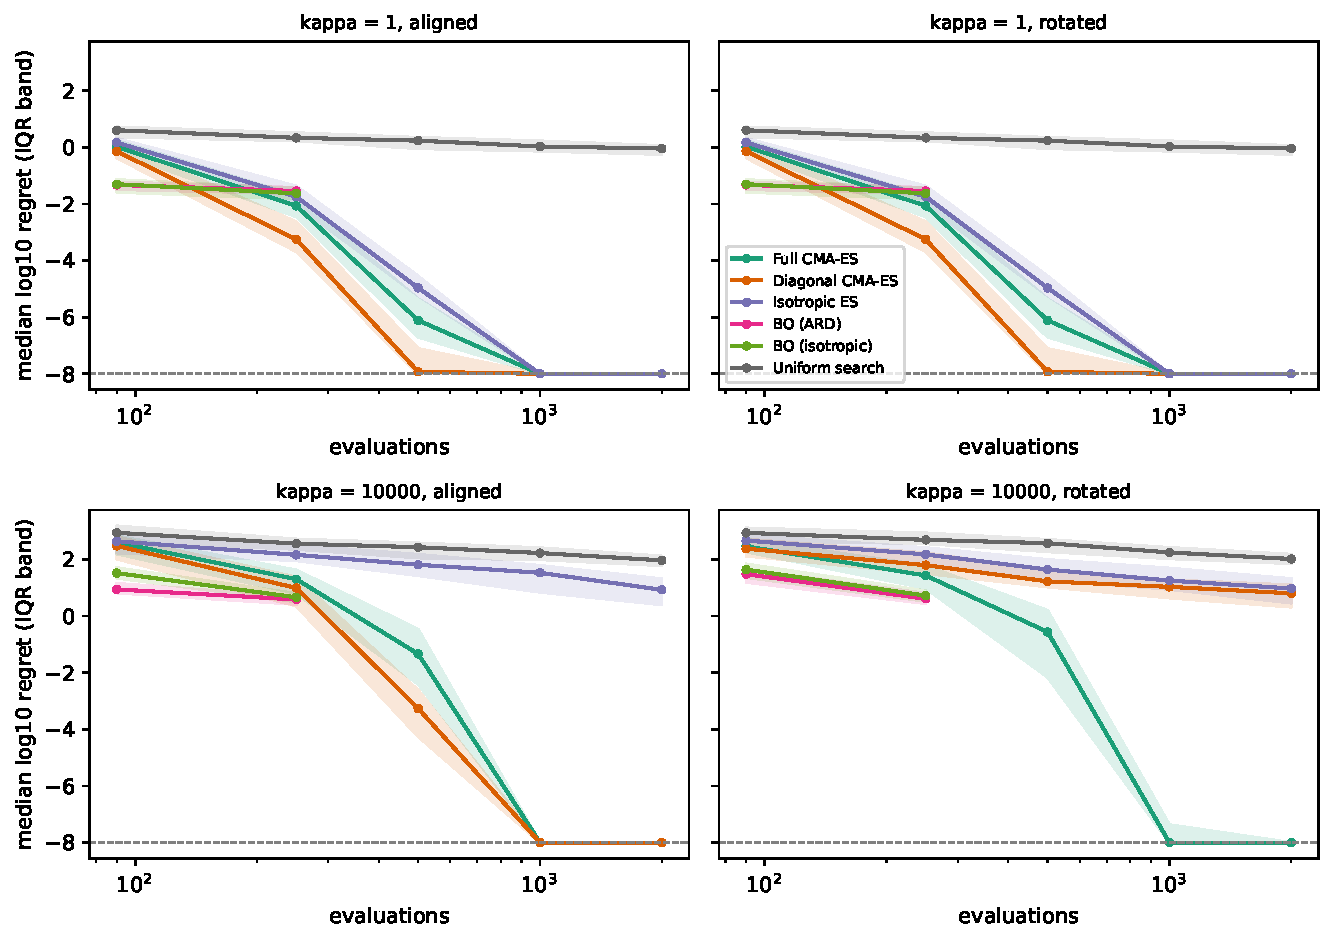
\includegraphics[width=0.72\textwidth]{figures/fig2_regret_curves.pdf}
\caption{Median log regret against evaluations (bands: interquartile range) at $\kappa=1$ (top) and $\kappa=10^4$ (bottom), aligned (left) and rotated (right). BO runs to 250 evaluations; the dashed line is the floor.}
\label{fig:curves}
\end{figure}

\begin{figure}[t]
\centering
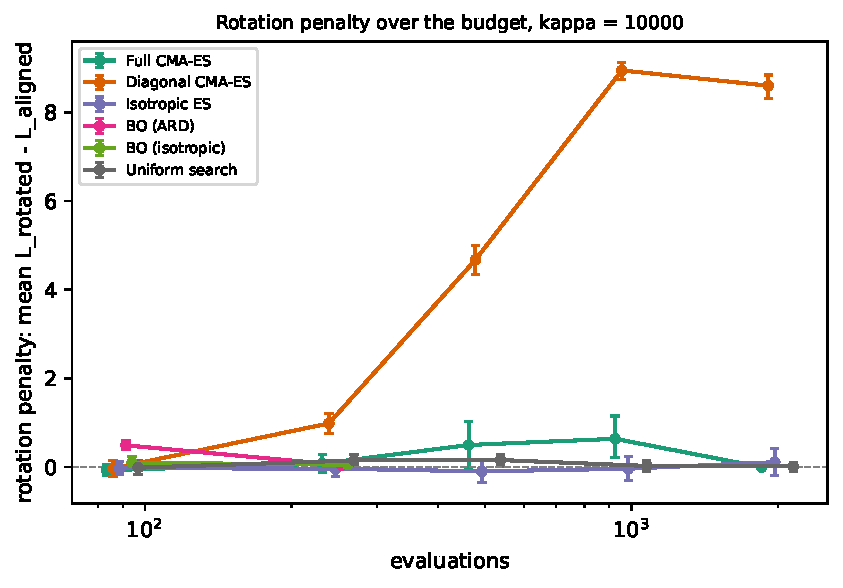
\includegraphics[width=0.52\textwidth]{figures/fig3_penalty_checkpoints.pdf}
\caption{Rotation penalty $\bar L_{\mathrm{rot}}-\bar L_{\mathrm{align}}$ at $\kappa=10^4$ against evaluations, with 95\% paired bootstrap intervals.}
\label{fig:penalty}
\end{figure}

\subsection{Mechanism}
The effective condition number shows what each method learned (Figure~\ref{fig:keff}). Full CMA-ES reduces $\kappa_{\mathrm{eff}}$ on the rotated problem from about 4{,}900 after 96 evaluations to 200 after 256 and 3.0 after 1{,}000. It settles at the same level on the trivial $\kappa=1$ problem (3.1), so a value of about 3 marks its practical floor rather than unlearned geometry. Diagonal CMA-ES reaches 2.5 when the problem is aligned but stays between about 6{,}500 and 8{,}500 throughout when it is rotated: it cannot learn the rotated shape. Isotropic ES stays at $\kappa=10^4$, as designed.

The pre-registered $\kappa_J$ test at $\kappa=10^4$ is null: across rotated instances, $\kappa_J$ does not predict the diagonal-minus-full gap ($\rho=-0.06\ [-0.35, 0.23]$). At $\kappa=10^2$ and $10^3$, where diagonal CMA-ES partly succeeds, the relationship is strong ($\rho=0.76\ [0.62, 0.86]$ and $0.63\ [0.42, 0.78]$). At $\kappa=10$ both methods reach the floor on every rotated instance, so the gap is zero and the correlation is undefined. For ARD BO, the fitted lengthscales at 250 evaluations follow the axis curvatures when the problem is aligned (median Spearman correlation with the axis weights $-0.77$) but not when it is rotated ($+0.23$).

\begin{figure}[t]
\centering
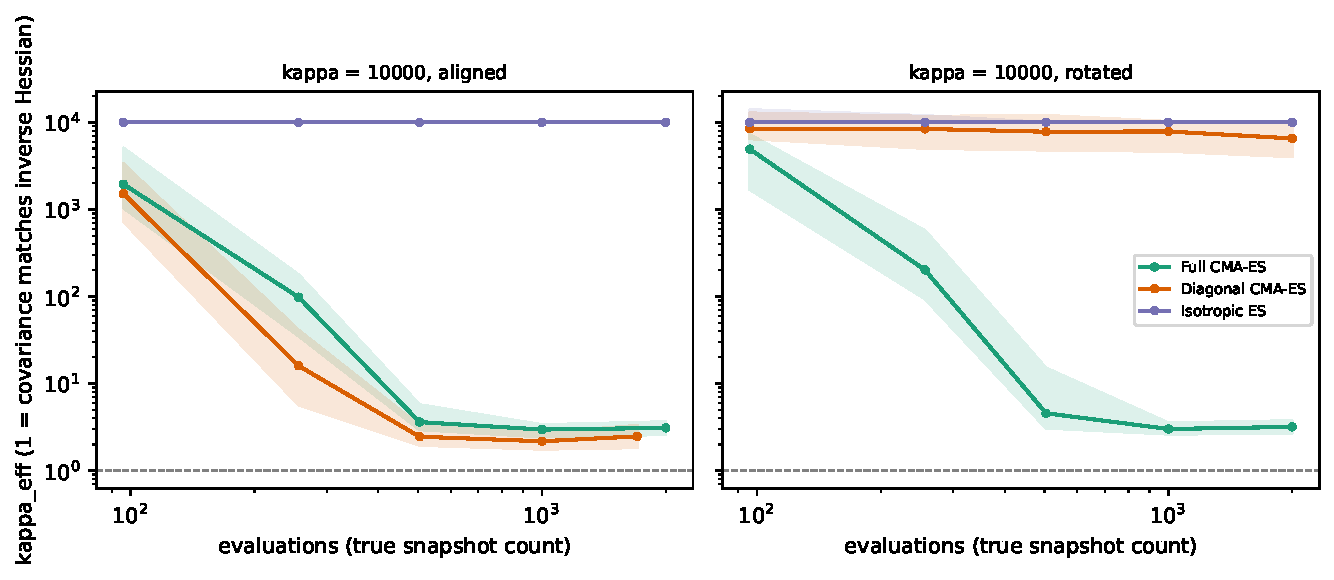
\includegraphics[width=0.72\textwidth]{figures/fig6_kappa_eff.pdf}
\caption{Median effective condition number $\kappa_{\mathrm{eff}}$ (bands: interquartile range) of the CMA-ES variants at $\kappa=10^4$, aligned (left) and rotated (right); 1 means the search distribution matches the inverse Hessian.}
\label{fig:keff}
\end{figure}

\subsection{Controls and validation}
At $\kappa=1$, aligned and rotated runs give the same regret for all six methods, to within $10^{-15}$, as expected: the rotated sphere is the same function, and the runs share their optimum, start and seeds. No run stopped for an unexpected reason: all 651 early stops were CMA-ES runs ended by pycma's numerical-precision checks. Bound repairs were rare (median at most 10\% of a run's evaluations, for isotropic ES on the rotated $\kappa=10^4$ problem). Uniform search matches its predicted success law at $\kappa=1$ (observed 0.06, 0.12, 0.28, 0.44 and 0.58 at the five checkpoints, against 0.04, 0.11, 0.22, 0.38 and 0.62). At $\kappa=10$, rotated, it succeeded more often than predicted at 1{,}000 and 2{,}000 evaluations (0.16 and 0.22 against 0.05 and 0.10), about three standard deviations, in one condition among about twenty informative comparisons; we report it without adjustment.

% ===================== 5 DISCUSSION =====================
\section{Discussion}
\label{sec:discussion}
\subsection{What the experiment establishes}
For the evolution strategies, the explanation is strongly supported. Rotation costs diagonal CMA-ES far more than full CMA-ES, the cost grows with conditioning, and the diagnostics show why: full CMA-ES learns the rotated shape ($\kappa_{\mathrm{eff}}\approx 3$) and diagonal CMA-ES cannot ($\kappa_{\mathrm{eff}}$ stays in the thousands). Two alternative readings are unlikely. The unrotated search box matters little, since uniform search, which has no model, shows a rotation penalty of at most 0.16; and full CMA-ES's own temporary penalty, which vanishes once it has adapted, matches the invariance-after-adaptation that theory predicts \parencite[p.~24]{hansen2023tutorial}. Rotation invariance therefore survives the practical implementation, with its bound handling and unrotated start, but only after adaptation. The pre-registered $\kappa_J$ test was null at $\kappa=10^4$. A likely reason, consistent with the strong correlations at $10^2$ and $10^3$, is that at $10^4$ every rotated instance leaves more conditioning than diagonal CMA-ES can handle within the budget, so differences in $\kappa_J$ no longer change the outcome; this is an interpretation, not a tested result.

For BO, the explanation is not supported at the comparison budget. ARD BO learned the axes when they were aligned (its lengthscales tracked the curvatures) and paid an early rotation penalty, but by 250 evaluations neither that penalty nor any difference from full CMA-ES or from isotropic BO ($-0.01\ [-0.14, 0.12]$) remained. What we can conclude is narrower: within 250 evaluations, ARD's axis-aligned model gives at most a short-lived advantage on aligned problems. Whether the effect would reappear at larger budgets, where full CMA-ES has adapted, could not be tested, because BO's cost limited it to 250 evaluations. BO nonetheless led in absolute terms at 250 evaluations, consistent with BO's strength at small budgets \parencite{raponi2023low}.

\subsection{Cost}
BO's advantage in evaluations comes at a large computational price: a 250-evaluation run took a median of 150--170\,s for ARD BO and 68--70\,s for isotropic BO, against about 0.2\,s for a 2{,}000-evaluation CMA-ES run. At $\kappa=10^4$, full CMA-ES needed a median of 330--368 evaluations to match the regret BO reached in 250, so BO pays off only if one evaluation costs more than about 1.4--1.9\,s (ARD) or 0.7--0.8\,s (isotropic); at $\kappa=1$, full CMA-ES matched BO in fewer evaluations, so BO never paid off. These times were measured on one laptop with eight runs in parallel and are indicative only.

\subsection{Limitations}
All methods use default settings, and BO is typically more sensitive to its settings than CMA-ES; its acquisition was also maximised without local refinement, to fit the compute budget. The study covers one function family, $d=4$ and $\kappa\le 10^4$, so it says nothing directly about multimodal, noisy or higher-dimensional problems; optional robustness checks over $\sigma_0$ and $d$ were not run. Regret at a fixed budget is a fixed-cost measure \parencite{hansen2009setup}, and the size of the diagonal-versus-full effect is set by the $10^{-8}$ floor, although its sign is not. Finally, uniform search succeeded more often than predicted in one condition ($\kappa=10$, rotated), which we report without adjustment.

% ===================== 6 CONCLUSION =====================
\section{Conclusion}
\label{sec:conclusion}
Rotating an ill-conditioned problem hurts a search method whose model is axis-aligned when the method cannot learn correlations: diagonal CMA-ES lost up to 8.6 orders of magnitude of regret relative to full CMA-ES, which learned the rotated geometry and became rotation-invariant once adapted. For Bayesian optimisation, an ARD kernel's axis-aligned model gave only a short-lived advantage on aligned problems, and within the 250 evaluations that its cost allowed it was no more sensitive to rotation than full CMA-ES. Testing BO at larger budgets, with cheaper surrogates, is the natural next step.

% ===================== REFERENCES =====================
\begin{multicols}{2}
\footnotesize            % if the list exceeds one page at the end, change to \scriptsize
\printbibliography
\end{multicols}

\end{document}